\documentclass[12pt]{article}

\usepackage[margin=1in]{geometry}

\usepackage{mathtools,amsthm}
\DeclarePairedDelimiter\ceil{\lceil}{\rceil}
\DeclarePairedDelimiter\floor{\lfloor}{\rfloor}

\usepackage{fontspec}
\newfontfamily\cmunicode{CMU Serif}
\usepackage{microtype}

\usepackage[noend]{algpseudocode}
\usepackage{algorithm}
\newcommand*\Let[2]{\State #1 $\gets$ #2}
\newcommand*{\TO}{\textbf{to}}
% since gemm3 can't be a matro name
\newcommand*{\pluseq}{\mathrel{{+}{=}}}
\newcommand*{\gemmt}{{\textsc{gemm3}}}
\newcommand*{\gemmtp}{{\textsc{gemm3()}}}
\newcommand*{\gemm}{{\textsc{gemm}}}
\newcommand*{\gemmp}{{\textsc{gemm()}}}

\newcommand*{\mycite}[1]{~\cite{#1}}

\usepackage{hyperref}
\usepackage{biblatex}

\addbibresource{cites.bib}

\usepackage{setspace}
%\singlespacing{}
\doublespacing{}

\usepackage{graphicx}

\usepackage{tikz}
\usetikzlibrary{arrows.meta,calc,fit,positioning,chains}
\definecolor{l3-color}{cmyk}{0,0.06,0.12,0}
\definecolor{l2-color}{cmyk}{0,0.2,0.4,0}
\definecolor{l1-color}{cmyk}{0,0.45,0.55,0}
\definecolor{reg-color}{cmyk}{0.15,0.8,0.8,0}

\tikzset{bpack/.style={to path={
      foreach \i in {1,...,#1} { -- ++(0.5, 0) -- ++ (-0.5,-0.4) } -- (\tikztotarget) \tikztonodes
    }},
  bpack/.default=6,
  apack/.style={to path={
      foreach \i in {1,...,#1} { -- ++(0, -0.5) -- ++(0.4,0.5) } -- (\tikztotarget) \tikztonodes
    }},
  apack/.default=6}

\tikzset{
  label-brace/.style={to path={
      (\tikztostart) ++(#1) -- ++(#1)
      -- ($(\tikztotarget) + 2 *(#1)$) \tikztonodes
      -- +($-1 *(#1)$)
    }},
  brace below/.style={label-brace={0, -3pt}},
  brace above/.style={label-brace={0, 3pt}},
  brace right/.style={label-brace={3pt, 0}},
  brace left/.style={label-brace={-3pt, 0}}}

\tikzset{
  dim-label/.style={label distance=0pt,inner sep=0},
}

\tikzset{
  our-arrow/.style={-{Latex[length=8pt,width=4pt]}},
}

\tikzset{
  memory/.style={fill=white},
  l3/.style={fill=l3-color},
  l2/.style={fill=l2-color},
  l1/.style={fill=l1-color},
  regs/.style={fill=reg-color},
  legend/.style={on chain=labels, minimum height=1ex, minimum width=1em,
    draw, rectangle, outer sep=0, label={[label distance=3pt]right:{\small #1}}}
}

\tikzset{
  loop-label/.style={midway, draw, rectangle},
  square-mat/.style={rectangle,draw,fit={(0, 0) (3, -3)},inner sep=0},
  wide-mat/.style={rectangle,draw,fit={(0, 0) (3, -1)},inner sep=0},
  tall-mat/.style={rectangle,draw,fit={(0, 0) (1, -3)},inner sep=0}
}

\newcommand*{\bpackarr}[2][6]{\draw[our-arrow] ($(#2 - 0.75, -0.25)$) to[bpack=#1] ++($(0.5, -0.4 * #1)$);}
\newcommand*{\apackarr}[2][6]{\draw[our-arrow] ($(0.25, - #2 + 0.75)$) to[apack=#1] ++($(0.4 * #1, -0.5)$);}

\newcommand*{\bracelabel}[4]{\draw (#1) to[brace #3]%
  node[midway,label={[dim-label]#3:#4}] {} (#2);}

\newcommand*{\packlabel}[3]{\path (#1) -- (#2)%
  node[midway,label={#3:pack}] {};}

% [style] name width height N code-for-every
\newcommand*{\vgrids}[6][fill=white]{
  \foreach \x in {1, ..., #5} {
    \node[rectangle, draw, #1,fit={($(#3 * \x - #3, 0)$) ($(#3 * \x, -#4)$)}, inner sep=0] (#2\x) {};
    #6
  }
}
% [style] name width height N code-for-every
\newcommand*{\hgrids}[6][fill=white]{
  \foreach \y in {1, ..., #5} {
    \node[rectangle, draw, #1,fit={($(0, -\y * #4 + #4)$) ($(#3, -\y * #4)$)}, inner sep=0] (#2\y) {};
    #6
  }
}

% [first-style] style name width height N code-for-every
\newcommand*{\vgridscache}[7][memory]{
  \foreach \x in {1, ..., #6} {
    \ifnum\x=1%
    \node[rectangle, draw, #1 ,fit={($(#4 * \x - #4, 0)$) ($(#4 * \x, -#5)$)}, inner sep=0] (#3\x) {};
    \else
    \node[rectangle, draw, #2 ,fit={($(#4 * \x - #4, 0)$) ($(#4 * \x, -#5)$)}, inner sep=0] (#3\x) {};
    \fi
    #7
  }
}
% [first-style] style name width height N code-for-every
\newcommand*{\hgridscache}[7][memory]{
  \foreach \y in {1, ..., #6} {
    \ifnum\y=1%
    \node[rectangle, draw, #1,fit={($(0, -\y * #5 + #5)$) ($(#4, -\y * #5)$)}, inner sep=0] (#3\y) {};
    \else
    \node[rectangle, draw, #2,fit={($(0, -\y * #5 + #5)$) ($(#4, -\y * #5)$)}, inner sep=0] (#3\y) {};
    \fi
    #7
  }
}

\newcommand*{\pluseqnode}[1]{\node[at={(0, -1.5)}] (#1-plus) {\large $\pluseq$};}

% [style] N N - 1 offset-right
\newcommand*{\loopborder}[3][black]{\draw[rounded corners, color=#1]%
  (#2-loop.west) -| ($(#3-rect-west) + (-5pt, -5pt)$) coordinate (#2-rect-west)%
  -- ($(#3-rect-east) + (5pt, -5pt)$) coordinate (#2-rect-east)%
  |- (#2-loop.east);}


\title{\gemmt{}: Constant-workspace high-performance multiplication of three matrices for matrix chaining}
\author{Krzysztof A. Drewniak}

\begin{document}
\maketitle{}
\section{Introduction}
The matrix chain problem asks how to efficiently parenthesize a matrix product $A_1A_2\cdots A_n$.
$O(n \log n)$ algorithms for solving this problem are known\mycite{Hu1984}, as are simpler $O(n^3)$ dynamic-programming solutions\mycite{Barthels2018}.
These algorithms all assume that the only operation available is the multiplication of two matrices.

In practice, a more general version of this problem appears, where matrices can be transposed and/or inverted, or have properties such as being upper triangular\mycite{Barthels2018}.
For example, an algorithm to compute the ensemble Kalman filter\mycite{Rao2017} (which computes parameters for physical systems from noisy data) requires the computation of the expression $X_i^b S_i (Y_i^b)^T R_i^{-1}$, which features one transposition and one inverse.
Other examples of the generalized matrix chain problem include the expression $L^{-1}AL^{-H}$ (where $L$ is lower triangular and $A$ is symmetric), which is knows as the two-sided triangular linear solve\mycite{Parikh2017} and $\tau_u\tau_v vv^TAuu^T$ (where the $\tau_i$ are scalars and $v$ and $u$ are vectors), which appears in an algorithm for reducing a matrix to tridiagonal form\mycite{Choi1995}.

The BLAS\mycite{blas_standard} and LAPACK\mycite{lapack_ug} libraries provide many high-performance functions that can assist in the computation of such matrix chains, such as specialized functions for the multiplication of triangular matrices (\textsc{trmm}()).
However, manually determining how to use these functions and coding in term of them requires expert knowledge.
Existing high-level systems, such at Matlab and Julia, which are commonly used by non-experts, generally compute generalized matrix chains in a naive way, such as proceeding from left to right, which is often ineffecient.
Systems such as Linnea\mycite{Barthels2017} have emerged recently that attack the generalized matrix chain problem and automatically generate a high-performance program for a given expression in term of high-performance operations such as matrix-matrix multiply.

Returning to the example matrix chains above, we can observe that they often contain the multiplication of three matrices as a subproblem, often after some preprocessing such as an inversion or an outer product.
The general form of such a problem is $G \coloneqq \alpha DEF + \beta G$ (with some of the operanrds optionally transposed), which we will summarize as $G \pluseq DEF$ and denote \gemmt{}, by analogy with the notation for general matrix-matrix multiply (\gemm{}) in the BLAS library.
The letters $D$, $E$, $F$, and $G$ were chosen to avoid confusion with discussions of \gemm{}, which has the form $C \pluseq AB$.
The only approach available for this subproblem with current methods is to paranthesize the expression $DEF$ and perform a pair of matrix multiplications, storing a result in a temporary matrix $T$.
This method has two drawbacks.
The first is that $T$ is often rather large (and could be larger than all the input matrices) and requires significant amounts of storage space.
In addition, if $T$ is sufficiently large, creating and using it incurs a non-negligible overhead due to the large number of slow main-memory operations required.

To combat these issues, we have developed an algorithm for \gemmt{} which does not require an entire intermediate product to be computed and stored at one time.
Our algorithm takes advantage of the blocking performed by modern \gemm{} implementations to only store a cache-sized block of $EF$ at any given time.
By doing so, we perform the multiplication in $O(1)$ additional space and maintain performance comparable with a pair of \gemm{} calls.
Our algorithm can therefore be used as a primitive in generalized matrix chain solvers (or hand-written matrix code) to reduce memory usage, decrease the complexity of the solution, and potentially provide a slight performance increase.

\section{Background}
\subsection{High-performance {\cmunicode \gemm{}}}
Before discussing our approach to \gemmt{}, it is important to review the implementation of high-performance \gemm{}.
High-performance \gemm{} algorithms operate by repeatedly reducing the multiplication to a series of multiplications of blocks of the inputs.
These blocks are sized to allow an operand to one of these subproblems to utilize a level of the CPU's cache effectively and prevent it from being evicted during further blocking.
Multiple levels of blocking are required to effectively utilize all levels of the cache.
These steps are necessary because of the memory hierarchy of modern CPUs, where there are multiple (currently three) levels of cache, which increase in size but decrease in speed, between registers and main memory.

There are two specialized primitives that appear in high-performance \gemm{}: the \emph{microkernel} and \emph{macrokernel}.
The microkernel is a highly-tuned, hand-written function (almost always implemented in assembly) that multiplies an $m_R \times k$ panel of $A$ by an $k \times n_R$ panel of $B$ to update an $m_R \times n_R$ region of $C$, which is updated in registers and written to memory.
An illustration of the microkernel is located in Algorithm \ref{alg:macrokernel}.
(In this illustration, as with all others in this work, constants that appear twice indicate the dimension along which each loop proceeds, along with the stride.)
The parameters $m_R$ and $n_R$ are based on the microarchitecture of the CPU, which can be derived analytically\mycite{Low2016} or by autotuning\mycite{Whaley1998}.

\begin{algorithm}
  \caption{The macrokernel of a high-performance \gemm{} implementation.}
  \label{alg:macrokernel}
  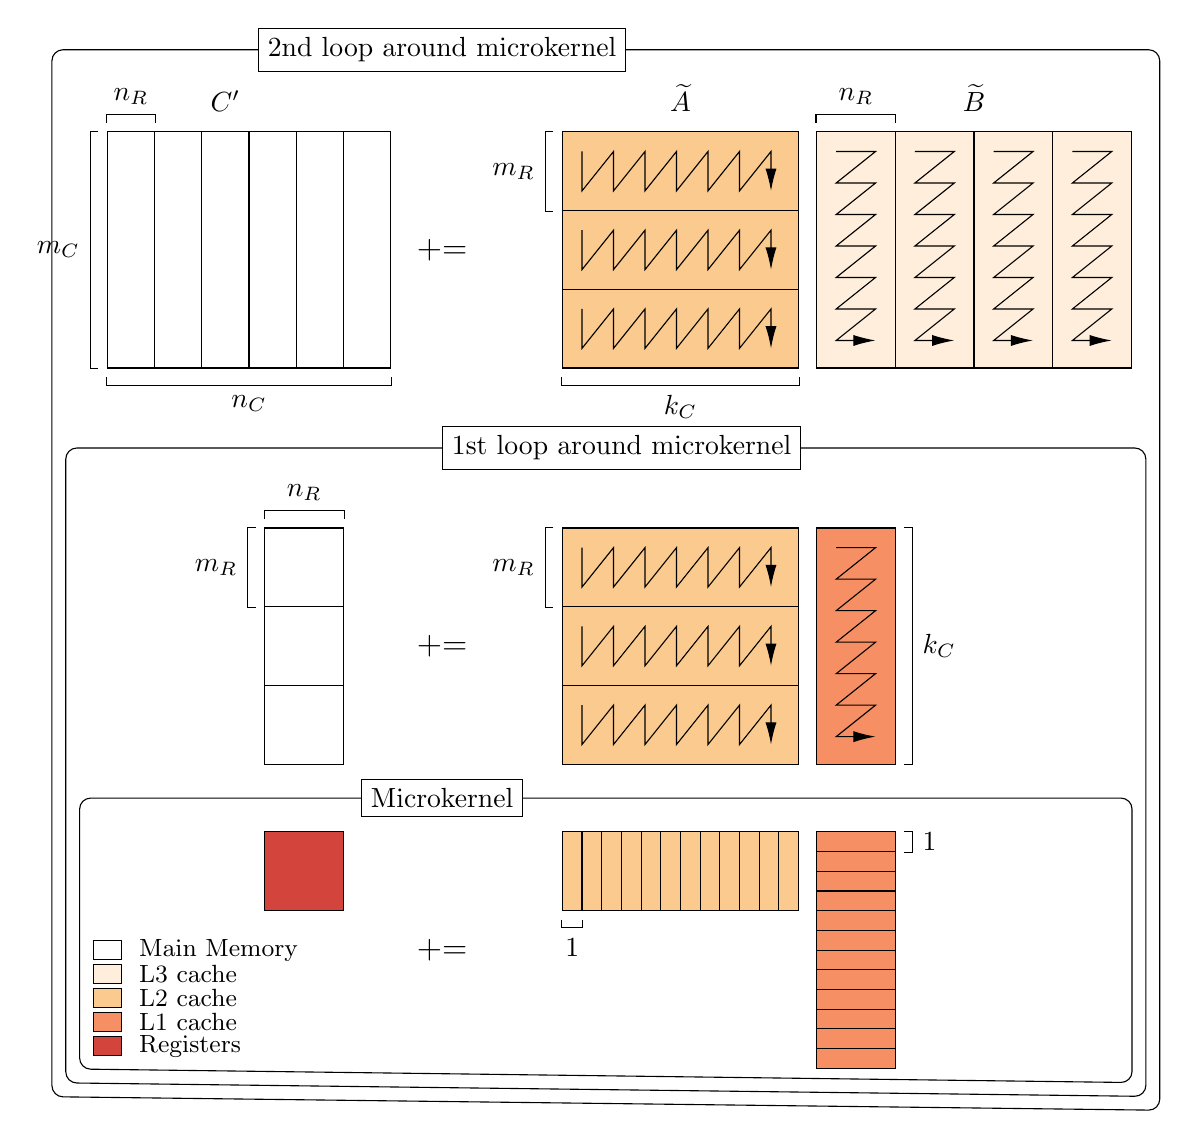
\begin{tikzpicture}
    \matrix (loops)[column sep=0.2cm, row sep=5.5ex] {
  \vgrids[memory]{2C}{0.6}{3}{6}{}
  \bracelabel{2C1.north west}{2C1.north east}{above}{$n_R$}
  \bracelabel{2C1.south west}{2C6.south east}{below}{$n_C$}
  \bracelabel{2C1.north west}{2C1.south west}{left}{$m_C$}
  \path (2C1.north west) -- (2C5.north east) node[midway,label={above:$C'$}] {};&

  \pluseqnode{2}&

  \hgrids[l2]{2A}{3}{1}{3}{\apackarr{\y}}
  \bracelabel{2A1.north west}{2A1.south west}{left}{$m_R$}
  \bracelabel{2A3.south west}{2A3.south east}{below}{$k_C$}
  \path (2A1.north west) -- (2A1.north east) node[midway,label={above:$\widetilde{A}$}] {};&

  \vgrids[l3]{2B}{1}{3}{4}{\bpackarr{\x}}
  \bracelabel{2B1.north west}{2B1.north east}{above}{$n_R$}
  \path (2B1.north west) -- (2B4.north east) node[midway, label={above:$\widetilde{B}$}] {};\\

  \foreach \y in {1,...,3} {
    \node[rectangle, draw, fit={(2, -\y + 1) (3, -\y)}, inner sep=0] (1C\y) {};
  }
  \bracelabel{1C1.north west}{1C1.south west}{left}{$m_R$}
  \bracelabel{1C1.north west}{1C1.north east}{above}{$n_R$}&

  \pluseqnode{1}&

  \hgrids[l2]{1A}{3}{1}{3}{\apackarr{\y}}
  \bracelabel{1A1.north west}{1A1.south west}{left}{$m_R$}&

  \vgrids[l1]{1B}{1}{3}{1}{\bpackarr{\x}}
  \bracelabel{1B1.north east}{1B1.south east}{right}{$k_C$}\\


  \node[rectangle, draw, regs, fit={(2, 0) (3, -1)}, inner sep=0] (0C) {};
  \begin{scoped}[start chain=labels going {below=2pt of \tikzchainprevious}]
    \node[legend=Main Memory, memory] at (0, -1.5) {};
    \node[legend=L3 cache, l3] {};
    \node[legend=L2 cache, l2] {};
    \node[legend=L1 cache, l1] {};
    \node[legend=Registers, regs] {};
  \end{scoped}&

  \pluseqnode{0}&

  \vgrids[l2]{0A}{0.25}{1}{12}{}
  \bracelabel{0A1.south west}{0A1.south east}{below}{$1$}&

  \hgrids[l1]{0B}{1}{0.25}{12}{}
  \bracelabel{0B1.north east}{0B1.south east}{right}{$1$}\\
};
\path node[draw,above=2cm of 2-plus] (2-loop) {2nd loop around microkernel}
(2-plus) -- (1-plus) node[loop-label,anchor=west] (1-loop) {1st loop around microkernel}
(1-plus) -- (0-plus) node[loop-label] (0-loop) {Microkernel};

\draw[rounded corners] let \p1 = ($(0B12.south east) + (0pt, -5pt)$),
\p2 = ($(2B4.south east) + (0pt, -5pt)$),
\p{east} = (\x2, \y1) in
(0-loop.west) -| ($(labels-end.south west) + (-5pt, -5pt)$) coordinate (0-rect-west)
-- (\p{east}) coordinate (0-rect-east)
|- (0-loop.east);

\loopborder{1}{0}
\loopborder{2}{1}

  \end{tikzpicture}
  \begin{algorithmic}
    \Procedure{macrokernel}{$\widetilde{A}, \widetilde{B}, C'$}
    \For{$j \gets 0, n_R, \ldots$ \TO{} $n_C$}
    \For{$i \gets 0, m_R, \ldots$ \TO{} $m_C$}
    \State{using the microkernel}
    \State{$C'[i:i + m_R, j:j + n_R] \pluseq \widetilde{A}[i:i+m_R,:] \cdot \widetilde{B}[:,j:j+n_R]$}
    \EndFor{}
    \EndFor{}
    \EndProcedure{}
  \end{algorithmic}
\end{algorithm}

In order for the microkernel to operate efficiently, the data within the panels must be arranged so that it is read in a linear fashion, which is the pattern of reads best suited to the CPU's memory prefetcher.
This is achieved by storing each panel of $A$ in column-major form with columns of height $m_R$ and keeping each panel of $B$ row-major with row width $n_R$.
This packed storage format in also illustrated in Algorithm \ref{alg:macrokernel}.

More importantly, to allow the microkernel to stream the data it operates on efficiently, the panels it examines must be stored in cache beforehand.
Since caches are fixed-size, we can only store a fixed number of such panels at any given time.
Specifically, we can only store an $m_C \times k_C$ block of $A$ and a $k_C \times n_C$ block of $B$.
The process of rearranging these blocks into the format needed by the microkernel is known as \emph{packing}.
The parameters $m_C$, $k_C$, and $n_C$ are chosen to ensure all levels of cache are used efficiently.

We will use $\widetilde{A}$ and $\widetilde{B}$ to denote the packed blocks of $A$ and $B$, respectively, and $C'$ to denote the corresponding block of $C$.
The loops that perform $C' \pluseq \widetilde{A}\widetilde{B}$ form the macrokernel, which is depicted as Algorithm \ref{alg:macrokernel}.
(In all the algorithms presented in this work, we will use Python-style notation for indexing, that is, matrices are 0-indexed and   $M[a:b, c:d]$ selects rows $[a, b)$ and columns $[c, d)$, with omitted operands spanning to the beginning/end of the dimension.)


Many high-performance \gemm{} implementations in use today are based on Goto's algorithm\mycite{Goto2008}.
One such implementation, which we have based our work on, is BLIS\mycite{VanZee2016}.
The BLIS algorithm, which is a refactoring of Goto's algorithm, is presented as Algorithm \ref{alg:blis}.
It brings a row panel of $B$ into the $L3$ (and later $L1$) cache, while storing a block of $A$ in $L2$.
\begin{algorithm}
  \caption{The BLIS algorithm}
  \label{alg:blis}
  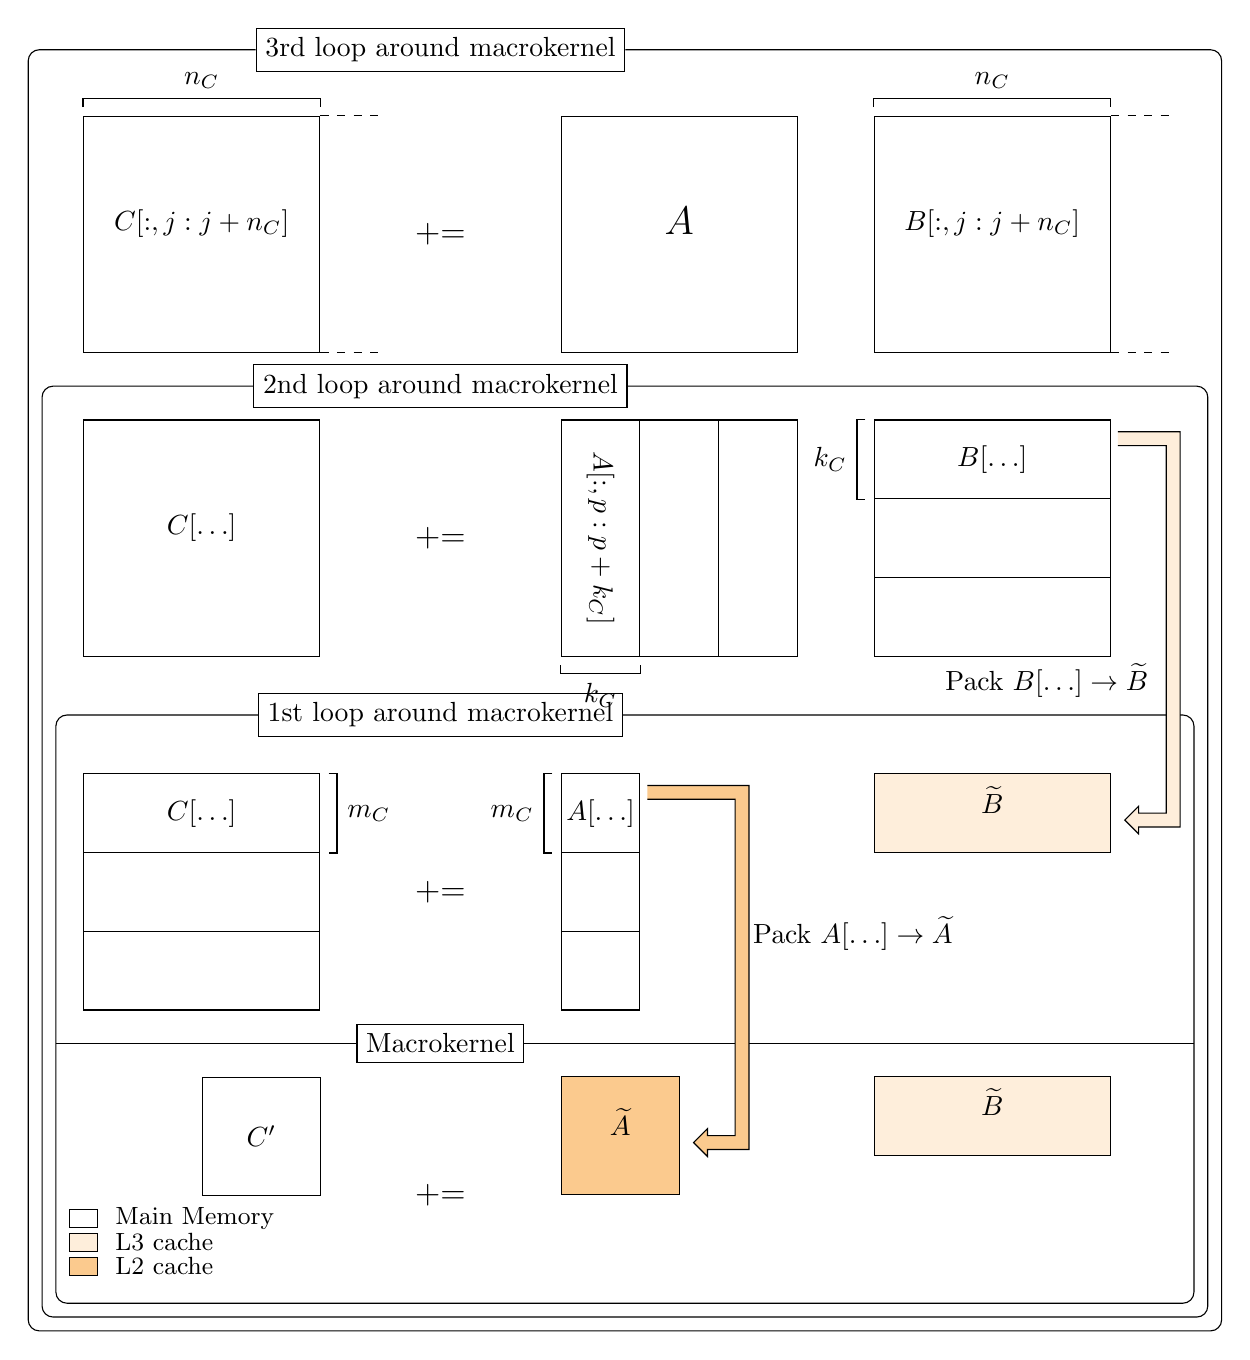
\begin{tikzpicture}
    \matrix (loops)[column sep=0.2cm, row sep=5.5ex] {
  \node[square-mat] (3C) {$C[:,j:j+n_C]$};
  \bracelabel{3C.north west}{3C.north east}{above}{$n_C$}
  \draw[dashed] (3C.north east) -- ++(0.75, 0)
  (3C.south east) -- ++(0.75, 0);&

  \pluseqnode{3}&

  \node[square-mat,memory] (3A) {\Large $A$};&

  \node[square-mat,memory] (3B) {$B[:,j:j+n_C]$};
  \bracelabel{3B.north west}{3B.north east}{above}{$n_C$}
  \draw[dashed] (3B.north east) -- ++(0.75, 0)
  (3B.south east) -- ++(0.75, 0);\\


  \node[square-mat,memory] (2C) {$C[\ldots]$};&

  \pluseqnode{2}&

  \vgrids[memory]{2A}{1}{3}{3}{}
  \node[at=(2A1),rotate=-90] {$A[:,p:p+k_C]$};
  \bracelabel{2A1.south west}{2A1.south east}{below}{$k_C$}&

  \hgrids[memory]{2B}{3}{1}{3}{}
  \node[at=(2B1)] {$B[\ldots]$};
  \bracelabel{2B1.north west}{2B1.south west}{left}{$k_C$}\\


  \hgrids[memory]{1C}{3}{1}{3}{}
  \node[at=(1C1)] {$C[\ldots]$};
  \bracelabel{1C1.north east}{1C1.south east}{right}{$m_C$}&

  \pluseqnode{1}&

  \hgrids[memory]{1A}{1}{1}{3}{}
  \node[at=(1A1)] {$A[\ldots]$};
  \bracelabel{1A1.north west}{1A1.south west}{left}{$m_C$}&

  \node[l3,wide-mat] (1B) {$\widetilde{B}$};\\

  \node[rectangle,draw,memory,at={(1.5, 0)},anchor=north west,minimum height=1.5cm, minimum width=1.5cm] (0C) {$C'$};
  \begin{scoped}[start chain=labels going {below=2pt of \tikzchainprevious}]
    \node[legend=Main Memory, memory] at (0, -1.8) {};
    \node[legend=L3 cache, l3] {};
    \node[legend=L2 cache, l2] (legend-anchor) {};
  \end{scoped}&

  \pluseqnode{0}&

  \node[l2,tall-mat,fit={(0, 0) (1.5, -1.5)}] (0A) {$\widetilde{A}$};&

  \node[l3,wide-mat,  wide-mat/.style={rectangle,draw,fit={(0, 0) (3, -1.5)},inner sep=0},] (0B) {$\widetilde{B}$};\\
};
\path node[draw,above=1.8cm of 3-plus] (3-loop){3rd loop around macrokernel}
(3-plus) -- (2-plus) node[loop-label] (2-loop){2nd loop around macrokernel}
(2-plus) -- (1-plus) node[loop-label] (1-loop) {1st loop around macrokernel}
(1-plus) -- (0-plus) node[loop-label] (0-loop) {Macrokernel};

\draw[rounded corners] let \p1 = ($(labels-end.south) + (0pt, -10pt)$),
\p2 = ($(0B.south east) + (30pt, 0)$),
\p3 = ($(labels-end.south west) + (-5pt, 0)$),
\p{east} = (\x2, \y1), \p{west} = (\x3, \y1) in
(1-loop.west) -| (\p{west}) coordinate (1-rect-west)
-- (\p{east}) coordinate (1-rect-east)
|- (1-loop.east);

\loopborder{2}{1}
\loopborder{3}{2}

\draw let \p1 = (0-loop),
\p2 = (1-rect-west),
\p3 = (1-rect-east),
\p{west-end} = (\x2, \y1),
\p{east-end} = (\x3, \y1) in
(0-loop.east) -- (\p{east-end})
(0-loop.west) -- (\p{west-end});

\path[draw, l3] (2B1.east) ++(2.5pt, 5pt) coordinate (B-arr-start)
-| ($(1B.east) + (20pt, 0pt)$) node[pos=0.82,left=3pt] {Pack $B[\ldots] \to \widetilde{B}$} coordinate (B-arr-down)
-- ++ (-10pt, 0)
-- ++(0pt, 2.5pt) -- ++(-5pt, -5pt) -- ++(5pt, -5pt) -- ++(0, 2.5pt)
-- ($(B-arr-down) + (5pt, -5pt)$)
|- ($(B-arr-start) + (0pt, 5pt)$);

\path[draw, l2] (1A1.east) ++(2.5pt, 5pt) coordinate (A-arr-start)
-| ($(0A.east) + (20pt, 0pt)$) node[pos=0.7,right=3pt] {Pack $A[\ldots] \to \widetilde{A}$} coordinate (A-arr-down)
-- ++ (-10pt, 0)
-- ++(0pt, 2.5pt) -- ++(-5pt, -5pt) -- ++(5pt, -5pt) -- ++(0, 2.5pt)
-- ($(A-arr-down) + (5pt, -5pt)$)
|- ($(A-arr-start) + (0pt, 5pt)$);

  \end{tikzpicture}
  \begin{algorithmic}
    \Procedure{BLIS\_gemm}{$A, B, C$}
    \For{$j \gets 0, n_C, \ldots$ \TO{} $n$}
    \For{$p \gets 0, k_C, \ldots$ \TO{} $k$}
    \State{pack $B[p:p+k_C,j:j+n_C] \to\widetilde{B}$}
    \For{$i \gets 0, m_C, \ldots$ \TO{} $m$}
    \State{pack $A[m:m+m_C,p:p+k_C] \to \widetilde{A}$}
    \State{$\textsc{macrokernel}(\widetilde{A}, \widetilde{B}, C[i:i+m_C,j:j+n_C])$}
    \EndFor{}
    \EndFor{}
    \EndFor{}
    \EndProcedure{}
  \end{algorithmic}
\end{algorithm}

\subsection{Parameter selection for the BLIS algorithm}\label{subsec:params}
The parameters $m_R$, $n_R$, $k_C$, $m_C$, and $n_C$ that appear in the BLIS algorithm are computed using an analytical model from \mycite{Low2016}.
We will summarize the process of deriving some of these parameters here.
The values of $m_R$ and $n_R$ determine the structure of the microkernel, and are derived from the width of vector registers on a given CPU along with the latency and throughput of fused-multiply-add (FMA) instructions.
Since we are reusing existing optimized microkernels, we will not detail the process of selecting these parameters except to note that $m_R$ and $n_R$ can be swapped during the cache-parameters selection process without sacrificing performance.

The process of selecting the remaining parameters assumes that, for each cache level $i$, the $L_i$ cache has is a $W_{Li}$-way set-associative cache with $N_{Li}$ sets and $C_{Li}$ bytes per cache line.
All the caches are also assumed to have a least-recently-used replacement policy.
$S_{elem}$ represents the size of a single element of the matrix for generality.

The first parameter we can derive is $k_C$, as it appears deepest in the loop structure of the algorithm.
We know that we will load a different $n_R \times k_C$ panel of $\widetilde{B}$ from $L1$ during each call to the microkernel.
We also know that the microkernel's reads from an $m_R \times k_C$ panel of $\widetilde{A}$ will cause it to be resident in the $L1$ cache.
Finally, some values from $C'$ will also enter the cache, and must not evict the panels.

To prevent the panels of $\widetilde{A}$ and $\widetilde{B}$ from evicting each other from the $L1$ cache, we want them to reside in different ways within each cache set.
To achieve this, the panels of $\widetilde{A}$ and $\widetilde{B}$ must both have sizes that are integer multiples of $N_{L1}C_{L1}$.
This restriction, along with the size of the data in each panel, tells us that
\begin{equation*}
  m_Rk_CS_{elem} = C_AN_{L1}C_{L1}
\end{equation*}
for some integer $C_A$, and that the same relationship holds for $n_R$ and $B$.

Given the three sources of data in the $L1$ cache, it must be the case that $C_A + C_B + 1 \leq W_{L1}$ (the $1$ is for elements of $C'$), and that we want to maximize $C_B$ given this constraint.
Therefore, we have
\begin{equation*}
  C_B = \ceil*{\frac{n_Rk_CS_{elem}}{N_{L1}C_{L1}}} = \ceil*{\frac{n_R}{m_R}C_A}
\end{equation*}
Manipulating the inequality further shows us that
\begin{equation*}
  C_A \leq \floor*{\frac{W_{L1} - 1}{1 + \frac{n_R}{m_R}}}
\end{equation*}

Choosing the largest possible value of $C_A$ that leaves $k_C$ an integer will maximize $k_C$, improving performance by increasing the amount of time spent in the microkernel.
It is as this point where $m_R$ and $n_R$ may need to be swapped.

Now that we have $k_C$, we can compute $m_C$ and $n_C$.
For $m_C$, we know that we need to reserve one way in the $L2$ cache for elements of $C'$, and $\ceil*{(n_Rk_CS_{elem})/(N_{L2}C_{L2})} = C_{B2}$ ways for the panel of $B$ in the $L1$ cache.
This allows us to bound $m_C$ by
\begin{equation*}
  m_C \leq \floor*{\frac{(W_{L2} - C_{B2} - 1)N_{L2}C_{L2}}{k_CS_{elem}}}
\end{equation*}
and then select $m_C$ as large as possible, keeping in mind that it must be divisible by $m_R$ for high performance.

Since the $L3$ cache is, in practice, very large and somewhat slow, $n_C$ is computed by finding the largest value such that $n_Ck_C$ is less that the size of the $L3$ cache, excluding an $L1$ cache's worth of space to allow elements of $C'$ or $\widetilde{A}$ to pass through.

\subsection{Data reuse in  matrix multiplication}
Examining the loops in the BLIS algorithm, as was done in\mycite{Low2016}, shows that each loop causes some data from the computation to be reused, that is, read or written it its entirety during each iteration of the loop.
For example, the micro-kernel reuses the small block of $C'$ that is stored in registers while looping over the panels.

Even though reuse occurs at each level of the algorithm, we will focus on the reuse of the packed buffers, as this is a key consideration for maintaining the performance of the algorithm\mycite{Henry92}.
Packing into $\widetilde{B}$ and $\widetilde{A}$ introduces overhead, time that is not usable for computation.
Therefore, reusing the packed buffers many times will lower the relative proportion of time spent on packing, thus increasing performance.

To improve reuse of $\widetilde{B}$, we need the first loop around the macrokernel, which packs into $\widetilde{A}$, to run many times, since each of those iterations covers computations that read the entirety of $\widetilde{B}$.
That is, we need $m$ to be large, as small values of $m$ will hurt performance by reducing the time between successive $\widetilde{B}$ packing operations.
Similarly, large values of $n$ allow the second loop around the microkernel to execute many times, thus improving reuse of $\widetilde{A}$, which is consumed by the first loop around the microkernel.

The only loops that iterate over $k$ are those that pack $\widetilde{B}$ (the second loop around the macrokernel) and the microkernel.
The second loop around the macrokernel does not result in the reuse of any data that has been loaded into cache because it is the first loop that performs such loads.
The microkernel only reuses data in registers, and so does not reuse cached data.
However, if $k$ is much less than $k_C$, the microkernel will only iterate a few times, increasing the proportion of time spent on non-computational overhaed.
Therefore, the size of $k$ has little impact on the reuse of packed blocks, except when $k \ll k_C$.

This reasoning shows that the BLIS algorithm achieves its best performance when $m$ and $n$ are large and $k$ is not extremely small.

\section{Algorithm}
For our discussion of \gemmt{}, we well be considering the operation $G \pluseq DEF$, where $D$ is $m \times k$, $E$ is $k \times l$ and $F$ is $l \times n$.

To derive our algorithm for \gemmt{}, we begin by considering the computation of $\textsc{gemm}(D, EF, G)$ with the BLIS algorithm, attempting to find ways to not need all of $EF$ at once.
We consider an execution of an \emph{outer algorithm} which computes $G \pluseq D(EF)$.
We then trace the execution of the outer algorithm, propagating any partitioning of $(EF)$ to a virtual computation of $(EF) = E \cdot F$.
This analysis demonstrated that no reads were performed from $(EF)$ until it was packed into $\widetilde{EF}$, and so we could defer packing it until then.

For $G \pluseq D(ED)$, the BLIS algorithm first partitions both $(EF)$ and $G$ in the $n$ dimension, creating the series of subproblems $G_{,1} \pluseq D(EF)_{,1}; G_{,2} \pluseq D(EF)_{,2}; \ldots; G_{,n \mod n_C} \pluseq D(EF)_{n \mod n_C}$.
These splits fix the $n$ dimension for each subproblem to be at most $n_C$.
When this partitioning is propagated to the virtual computation of $EF$, the corresponding subproblems have the form $(EF)_{,j} \pluseq EF_{,j}$.

Then, for each of the subproblems (we will consider the $j$th one here), the outer algorithm partitions in the $k$ dimension with a stride of $k_C$.
The resultant subproblems are $G_{,j} \pluseq D_{,1}(EF)_{1,j}; G_{,j} \pluseq D_{,2}(EF)_{2,j}; \ldots; G_{,j} \pluseq D_{,k \mod k_C}(EF)_{k \mod k_C,j}$, which correspond to the virtual subproblems $(EF)_{i,j} = E_{i,}F_{,j}$.

In the outer algorithm, the next step would be to pack $(EF)_{i,j}$ into $\widetilde{EF}$, which requires elements of $(EF)$ to be available.
Therefore, we must turn to the problem of finding an \emph{inner algorithm} for this subproblem.
Such an algorithm would multiply a  $k_C \times l$ row panel of $E$ by an $l \times n_C$ block (or, eventually, column panel) of $F$ to produce a $k_C \times n_C$ row panel of $EF$.
Per our discussion of matrix reuse, such a shape can be computed by the BLIS algorithm without incurring serious efficiency problems.

The output of any such inner algorithm fits in a buffer of $k_Cn_C$ floating-point numbers, which takes $O(1)$ space, as opposed to the $O(kn)$ space needed to compute $(EF)$ in its entirety.
Therefore, we can improve memory usage while maintaining performance by only computing elements of $(EF)$ before the packing step of the outer algorithm.
Computation earlier in the algorithm would not retain these benefits, and so this choice was necessary to ensure the properties we sought.

An initial approach to implementing the inner algorithm $EF_{i, j} = E_{i,}F_{,j}$ would be to reuse the BLIS algorithm, nesting it within the outer computation.
This nesting would, at first, create a redundant outer loop in the inner algorithm, since $n$ cannot be more than $n_C$ for these subproblems
However, even with the outer loop removed, this naive approach caused performance issues.
One such issue was that there was no guarantee that the inner algorithm (which computes blocks of $EF$) would place its results into cache.
Another difficulty came from the fact that we would still need to pack blocks of $EF$ into $\widetilde{EF}$, incurring a cost in memory operations we hoped to avoid.

Fortunately, these problems are resolvable.
The microkernel can be made to write in the packed format, eliminating a large number of memory operations, by informing it that the output matrix was row-major with rows of width $n_R$.
To solve the cache-residency issue, we observed that, if we used an $n_C$ value that was half of the one from BLIS, both a packed block of $F$ and the output block of $EF$ could reside in the $L3$ cache simultaneously.
This change does not break the assumptions of the BLIS algorithm, as $n_C/2$ is still much larger than $k_C$ or $m_C$ in practice.

Another issue with this approach is that the inner computation is a panel-matrix multiply, that is, the $m$ dimension is small, and $\widetilde{F}$ would see little reuse.
This suboptimal shape did have a performance impact, though it turned out to be small in practice.

There was one other adjustment made to the BLIS algorithm's parameters in order to to enable the fusion to remain efficient.
In some cases, the BLIS microkernel's loops have a final iteration that considers fewer than $m_R$ rows (or $n_R$ columns) because not all matrices have sizes divisible by $m_R$ and $n_R$.
Computation of this fridge iteration can have a performance impact, as special processing is required to account for the unusual sizes.
In the fused BLIS algorithm, the value of $k_C$ becomes the $m$ dimension of the problem computed by the inner algorithm.
If $k_C$ is not divisible by $m_R$, we must, at the cost of slightly less optimal cache usage, reduce it slightly so that it is a multiple of $m_R$, thus ensuring we do not incur performance penalties every time we compute $\widetilde{EF}$.
However, $l_C$, which is the inner algorithm's version of $k_C$, can be kept at the BLIS value, as these considerations are not relevant there.

The algorithm that resulted from this derivation is Algorithm \ref{alg:gemm3}, which is illustrated in Figure \ref{fig:gemm3}.

\begin{figure}
  \centering
  \includegraphics[height=8.75in]{gemm3-picture}
  \caption{Illustration of algorithm for \gemmt{}. Constants that appear twice indicate the dimension along which each loop proceeds, along with the stride.}
  \label{fig:gemm3}
\end{figure}
\begin{algorithm}
  \caption{Algorithm for \gemmt{}}
  \label{alg:gemm3}
  \begin{algorithmic}
    \Procedure{gemm3}{$D, E, F, G$}
    \For{$j \gets 0, n_C, \ldots$ \TO{} $n$}
    \For{$p \gets 0, k_C, \ldots$ \TO{} $k$}
    \For{$q \gets 0, l_C, \ldots$ \TO{} $l$}
    \State{pack $F[q:q+l_C,j:j+n_C] \to \widetilde{F}$}
    \For{$i \gets 0, m_C, \ldots$ \TO{} $k_C$}
    \State{pack $E[i:i+m_C,q:q+l_C] \to \widetilde{E}$}
    \State{$\textsc{macrokernel}(\widetilde{E}, \widetilde{F}, \widetilde{EF})$}
    \Comment{writes in packed form}
    \EndFor{}
    \EndFor{}
    \For{$i \gets 0, m_C, \ldots$ \TO{} $m$}
    \State{pack $D[m:m+m_C,p:p+k_C] \to \widetilde{D}$}
    \State{$\textsc{macrokernel}(\widetilde{D}, \widetilde{EF}, G[i:i+m_C,j:j+n_C])$}
    \EndFor{}
    \EndFor{}
    \EndFor{}
    \EndProcedure{}
  \end{algorithmic}
\end{algorithm}

It should be noted that this algorithm computes $G \pluseq D(EF)$.
In some cases, it is much more efficient (on account of the dimensions of the inputs) to compute $G \pluseq (DE)F$ instead.
Attempting to derive an algorithm for that problem directly does not work, as the block $\widetilde{DE}$ in $L2$ is not of a shape that can be multiplied efficiently by the BLIS algorithm.
Fortunately, we can transform problems of this form to the equivalent problem $G^T \pluseq F^T(E^TD^T)$.
This transformation can be performed at effectively no cost by re-interpreting the memory the matrices are stored in (treating a row-major matrix as column-major and vice-versa).

\section{Experiments and Results}
To test our algorithm's performance, we implemented both it and the BLIS algorithm in the Multilevel Optimization for Matrix Multiply Sandbox (MOMMS), which wes developed for\mycite{SmithDiss2017}.
This framework allowed us to declaratively generate the code for an algorithm by specifying the series of loops and packing operations required, and allowed us to interface to the BLIS microkernels.
Initially, we verified that the MOMMS implementation of the BLIS algorithm had similar performance to the reference implementation, which was written in C.

We modified the framework to add support for ``subcomputations'', which are virtual objects that represent a \gemm{} operation.
Subcomputations pass through partitionings to their respective input matrices, and then can be forced to fill a given output matrix.
This both allowed us to cleanly express the \gemmt{} algorithm, and allowed the typical $T = EF; G \pluseq DT$ algorithm for \gemmt{} to be expressed as the BLIS algorithm where one operand is the BLIS algorithm as a subcompuation, with that operand being forced immediately.

We tested the performance, in gigaflops per second, of both our algorithm and the typical approach.
The experiments were run on a public lab machine at the University of Texas at Austin.
The machine had an Intel Xeon E3-1270 v3 CPU, which ran at 3.5 GHz and implemented the Haswell microarchitecture.
The experimental system had 15 GB of RAM, 8 MB of $L3$ cache, 256 KB of $L2$ cache (which was an 8-way set-associative cache with 64 byte cache lines) and $32 KM$ of $L1$ cache (per core), which had the same characteristics as the $L2$.
The blocking parameters that arose from this data can be found in Table \ref{tab:parameters}

\begin{table}
  \centering
  \begin{tabular}{l|c c}
    &\gemmt{}&BLIS algorithm\\ \hline
    $m_C$&72&72\\
    $k_C$&252&256\\
    $l_C$&256&\\
    $n_C$&2040&4080\\
  \end{tabular}
  \caption{Blocking parameters for Haswell}
  \label{tab:parameters}
\end{table}

Our experiments were run both on square matrices ($m = n = k = l = N$) and on problems where a particular dimension was fixed at $9$ while the others varied together, to evaluate the performance of these algorithms on multiple input shapes.
We sampled the performance at multiples of sixteen from $N = 16$ to $4912$ to test the suitability of our approach on many input sizes.
All the inputs were stored column-major, while the temporaries and outputs were stored row-major, since the BLIS microkernel has noticably increased performance when writing to row-major matrices (and since the packed buffer is row-major).
This unusual combination of input formats ensured a fair comparison between the two algorithms.
In addition, we tested the $G^T = F^T(E^TD^T)$ case, in which all matrices were row major, for square inputs.

The results of these experiments can be found in Figure \ref{fig:bc_square} for square matrices, and Figure \ref{fig:bc_rectangles} for the rectangular inputs.
The $G \pluseq (DE)F$ experiment's results are in Figure \ref{fig:ab_square}.
Data for the square case shows that, once performance has stabilized around $N = 512$, the two algorithms are almost always within 5\% of each other in GFlops/s, showing comparable performance.

\begin{figure}
  \centering
  \includegraphics[height=0.40\textheight]{../results/earwig2/gemm3}
  \caption{Performance of our \gemmt{} implementation compared to a pairr of \gemm{} calls, square matrices}
  \label{fig:bc_square}
\end{figure}

\begin{figure}
  \centering
  \includegraphics[height=0.40\textheight]{../results/earwig2/gemm3_rectangles}
  \caption{Performance of our \gemmt{} implementation compared to a pairr of \gemm{} calls, rectangular matrices}
  \label{fig:bc_rectangles}
\end{figure}

\begin{figure}
  \centering
  \includegraphics[height=0.40\textheight]{../results/earwig2/gemm3_ab_bc_kernel}
  \caption{Performance of our \gemmt{} implementation compared to a pairr of \gemm{} calls, square transposed matrices}
  \label{fig:ab_square}
\end{figure}

The computed additional (excluding inputs and outputs) memory consumption of both algorithms for square matrices of various input sizes is shown in Figure \ref{fig:bc_square_mem}, demonstrating our approach's much lower memory usage.
\begin{figure}
  \centering
  \includegraphics[height=0.40\textheight]{../results/earwig2/gemm3_memory}
  \caption{Memory usage of our \gemmt{} implementation compared to a pairr of \gemm{} calls}
  \label{fig:bc_square_mem}
\end{figure}

\section{Discussion}
From the figures in the previous section, it is clear that \gemmt{} attains similar performance to a pair of \gemm{} calls with significantly lower memory usage.
However, it is important to dissect these performance results and determine why they have arisen.

For the square case, which was shown in Figure \ref{fig:bc_square}, we can observe that, for most of the 1000s and 2000s, the pair of \gemm{} calls has somewhat increased performance, but that the \gemmt{} algorithm is comparably or even more performant afterwards.
The higher performance for the \gemm{} calls arises from the lack of reuse of $\widetilde{C}$ implied by the $252 \times l \cdot l \times n$ input to the inner algorithm for \gemmt{}.
Specifically, the first loop around the macrokernel in that algorithm always iterates at most four times, compared to the unbounded number of iterations in a call to \gemm{} to compute $EF$.
However, around when the temporary grows to 64 MB, the memory cost of writing it to memory becomes large enough that the performance of two \gemm{} calls begins to drop to and eventually falls below the performance of our \gemmt{} algorithm.
This shows that our approach, in addition to the memory savings, provides performance benefits for large matrix multiplications.

For small input sizes ($N < 512$), there is often a significant performance benefit attained by the \gemmt{} algorithm.
This performance improvement arises from the additional packing step that a pair of \gemm{} calls must perform, which has a non-negligible cost for these inputs, even if both the packed and unpacked data remain resident in the $L3$ cache.

Similar trends can be seen in Figure \ref{fig:ab_square}, which shows the results for $G \pluseq (DE)F$, implemented as $G^T \pluseq F^T(E^TD^T)$.
However, the pair of \gemm{} calls retains higher performance for a longer period of time on this workload.
This occurs because packing from row-major matrices to row-major packed buffers, which is something that occurs more frequently in this experiment, is much more amenable to the CPU's prefetcher than packing from column-major matrices.

The rectangular results from Figure \ref{fig:bc_rectangles} also require examination.
When $l$ is small, the \gemmt{} algorithm performs better on all inputs, as the memory-writing overhead in the BLIS algorithm remains, while the advantage of reuse in computing $EF$ is reduced (because the $k$ dimension is very narrow).
When $m$ is small, the costs of low $L3$ reuse are imposed at least once on both algorithms, decreasing the performance of both.

When $n$ is narrow, the problem is effectively converted to a series of several matrix-vector multiplications, which cannot achieve high performance with either algorithm.
For narrow $k$, the outer problem is an outer product, while the inner problem is a panel-matrix multiply (wide matrix times square matrix).
These shapes do not generally promote data reuse within the BLIS algorithm.
The eventually increased performance of \gemmt{} with $k = 9$ is due to the lowered number of memory operations that algorithm performs, since memory operations dominate this computation.

These results demonstrate the general suitability of our algorithm for \gemmt{} and its suitability as a high-performance primitive.

\section{Things that still might need doing}
\begin{itemize}
\item Portability (run on KNL)
\item Clean experiments (public lab machines are kinda a bad place)
\item Parallel case (the square-case performance behavior we have is still there, just much more exaggerated on multiple cores)
\item Make this somewhat longer to keep the writing flag people happy (should happen if we fix one of these other points)
\end{itemize}
\printbibliography{}
\end{document}
